\documentclass[12pt,a4paper]{article}
\usepackage[utf8]{inputenc}
\usepackage[english]{babel}
\usepackage[T1]{fontenc}
\usepackage{amsmath}
\usepackage{amsfonts}
\usepackage{amssymb}
\usepackage{graphicx}
\usepackage{titlesec}
\usepackage[left=2cm,right=2cm,top=2cm,bottom=2cm]{geometry}
\usepackage{indentfirst}
\usepackage{listings}
\usepackage{color}
\usepackage{url}
\usepackage{array}

%Pravidlo pro řádkování
\renewcommand{\baselinestretch}{1.5}

%Pravidlo pro začínání kapitol na novém řádku
\let\oldsection\section
\renewcommand\section{\clearpage\oldsection}

%Formáty písem pro nadpisy (-změněno na bezpatkové \sffamily z původního \normalfont
\titleformat{\section}
{\sffamily\Large\bfseries}{\thesection}{1em}{}
\titleformat{\subsection}
{\sffamily\large\bfseries}{\thesubsection}{1em}{}
\titleformat{\subsubsection}
{\sffamily\normalsize\bfseries}{\thesubsubsection}{1em}{}

%Nastavení zvýrazňování kódu v \lslisting
\definecolor{mygreen}{rgb}{0,0.6,0}
\definecolor{mygray}{rgb}{0.5,0.5,0.5}
\lstset{commentstyle=\color{mygreen},keywordstyle=\color{blue},numberstyle=\tiny\color{mygray}}

\author{Štěpán Ševčík}

\begin{document}

%-------------Úvodni strana---------------
\begin{titlepage}


\includegraphics[width=50mm]{img/FAV.jpg}
\\[160 pt]
\centerline{ \Huge \sc KIV/FJP - Formal Languages and Compilers}
\centerline{ \huge \sc Semestral project}
\\[12 pt]
{\large \sc
\centerline{Crest generation from Blazon}
}


{
\vfill 
\parindent=0cm

\begin{center}
\begin{tabular}{|c | c | c |}
	\hline
	\textbf{Name} & \textbf{Student number} & \textbf{E-mail} \\ \hline
	Jan Vampol & A17N0028P & \\ \hline
	Štěpán Ševčík &  A17N0087P & kiwi@students.zcu.cz \\ \hline
	Zdeněk Valeš & A17N0094P & \\ \hline
\end{tabular}
\end{center}
\textbf{Date:} {\large \today\par} %datum
\textbf{Repository:} \url{https://github.com/Thoronir42/heraldry}

}

\end{titlepage}

%------------------Obsah-------------------
%\newpage
%\setcounter{page}{2}
%\setcounter{tocdepth}{3}
%\tableofcontents
%------------------------------------------

%--------------Text dokumentu--------------


\section{Abstract}
In the medieval heraldry, blazon is used to describe war symbols such as a coat of arms or a similar emblems. If understood as a formal language, blazon can be processed and to a certain level automatically compiled and rendered into an appropriate visual or text representation.

\section{Introduction}
During the medieval ages the best way to resolve disputes was often by force and the greater the force is, the trickier it is to control. The form of force this article explores is an army made of hundreds to thousands of soldiers. In order for armies to represent a country or a clan, it needs to be exactly defined in order to be easily recognized. For this reason blazon was invented, which is a strict language originally built on the old English.
Blazon is used to describe various parts, each representing certain aspect of given arms. The most expressive part is the \textbf{coat of arms}, or in other words the shield, which displays main properties or feats of the arms.
While there are other parts such as the supporters, crest, helmet and more, this article focuses on the coat of arms and examines methods of processing of the blazon.

This article briefly introduces the formal languages and grammars defining them which will help with understanding the transformation process. Then the blazon language is examined and its elements described and finally the process transforming blazon into corresponding visual representation.

\section{Assignment}
The goal of this project is to:
\begin{itemize}
\item formalize blazon into a formal language,
\item design grammar,
\item at least partially implement generator functionality allowing rendition of a crest.
\end{itemize}

\subsection{Analysis}
The blazon language is constructed upon a variety of spoken languages, such as English, Scottish, Czech, German, etc...
For this reason, it was chosen to construct the terminal symbols through vocabularies in form of \textit{comma separated values} files which are composed into a \textbf{Vocabulary} structure.

\section{Blazon}
The emergence of heraldry as we know it today was linked to the need to distinguish participants quickly and easily in combat \cite{InternationalHeraldry}.
While quick distinction in battle is the primary reason for blazoning, it's also used as a way to display achievements or clan relations.

Blazon accomplishes this using various elements which in matter of speaking are working together as a building kit. The root of a coat of arms is a field, which can be in a simplest case defined by a Tincture, which is either a solid colour, metallic colour or a pattern called fur. The most common Tinctures are depicted on the Figure \ref{tinctures}. The Rule of Tincture prohibits certain colour combinations although in some cases it is broken intentionally.
\begin{figure}[h]
	\centering
	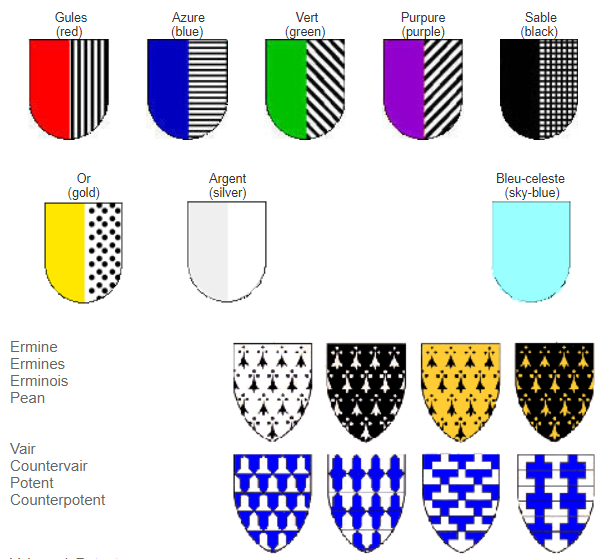
\includegraphics[width=80mm]{img/tinctures.png}
	\caption{Most common tinctures used in blazon \cite{InternationalHeraldry}}
	\label{tinctures}
\end{figure}

In the early days of heraldry, very simple bold rectilinear shapes were painted on shields. These are called ordinaries or sometimes "honourable ordinaries" as they could be easily recognized at a long distance and could be easily remembered.
They therefore served the main purpose of heraldry—identification. \cite{InternationalHeraldry}

\begin{figure}
	\centering
	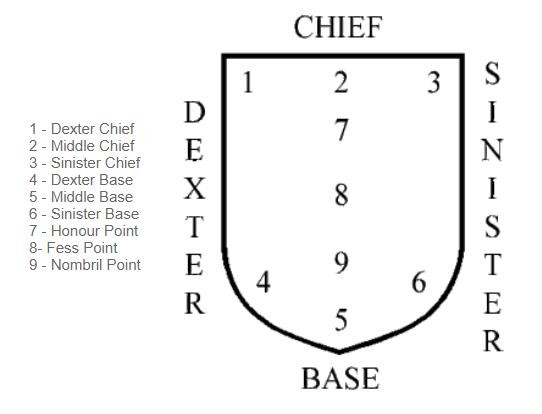
\includegraphics[width=0.5\linewidth]{img/locations}
	\caption{Locations on Coat of Arms}
	\label{fig:locations}
\end{figure}
Any object ranging from simplest shapes to mythical animals can be placed in a field in a role of a Charge.
Sometimes a coat of arms can be introduced as a Charge which usually represents heritage or conjunction of arms and when done so, this inner coat of arms is called inescutcheon.
\pagebreak

Besides placement on a field, charges can be also placed on top of charges or in a one of the locations in chief, on top, or in base, on the bottom, of the shield.
In these locations horizontal alignment can be specified from viewers left to right: Dexter, Middle and Sinister.
These locations and some special points are depicted on Figure \ref{fig:locations}.

Another way of creating more variations is to vary the field. The field can be divided into more than one tincture.
Many coats of arms consist simply of a division of the field into two contrasting tinctures. \cite{InternationalHeraldry}

Few examples of ways to divide the field are split in half vertically "party per pale", split in half horizontally "partly per bend" or split quarterly. These and few more examples are shown on Figure \ref{fig:fielddivisions}.
\begin{figure}[h]
	\centering
	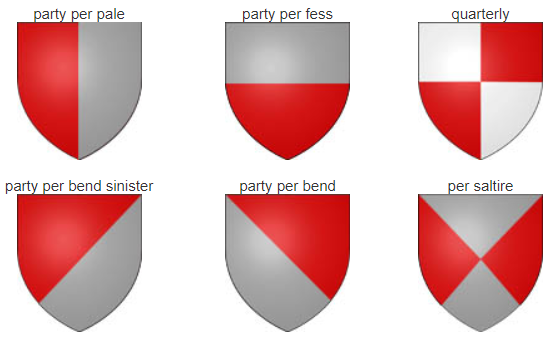
\includegraphics[width=0.60\linewidth]{img/fieldDivisions}
	\caption{Field division examples}
	\label{fig:fielddivisions}
\end{figure}

Portions of field divisions become new fields which are described in same manner as the whole coat of arms in order, unless specified otherwise, from top to bottom, from left to right.

\subsubsection{Example blazon}
An example of blazoned Arms of Churchill as seen on Figure \ref{armsOfChurchillImg} shows usage of various elements such as the quarterly division of field, escallops and lion charges or inescutcheon augmentation:

Quarterly 1st and 4th Sable a lion rampant on a canton Argent a cross Gules;
2nd and 3rd quarterly Argent and Gules in the 2nd and 3rd quarters a fret Or overall on a bend Sable three escallops of the first and as an augmentation in chief an inescutcheon, Argent a cross Gules and thereon an inescutcheon Azure, three fleurs-de-lis Or.
\begin{figure}[h]
	\centering
	
\includegraphics[width=50mm]{img/512px-Arms_of_Winston_Churchill.png}
	\caption{Arms of Churchill rendered \cite{ArmsOfChurchillImg}}
	\label{armsOfChurchillImg}
\end{figure}

In this example, there can be seen a quarterly division being used with field repetition using the ordinal numbers specifying which fields are being described. Placement of inescutcheon in chief and another inescutcheon within is also demonstrated.

\section{Formal language}
In order to define a formal language, we need to understand the parts it is composed of - the words and the alphabet.
A word (or string) is a finite sequence of items, so-called symbols or letters chosen from a specified finite set called the alphabet.
Examples of common alphabets are e.g. letters in the Latin alphabet (+ interword space, punctuation marks, etc.), and the bits 0 and 1.\cite{ruohonen2009formal}
By definition formal language is a set of words over some alphabet and in other words, formal language is a rule set enumerating possible combinations of words that are.

Current implementation of blazon consists of 15 non-terminal symbols, which are directly rewritten into terminals.

These symbols are:
\begin{itemize}
\setlength\itemsep{-0.5em}
\item \textbf{Tincture (15)} A color or fur-like material,
\item \textbf{Field division(11)} Mean of dividing a field,
\item \textbf{Field variation(9)} Filling pattern definition,
\item \textbf{Division line(9)} Style of dividing line,
\item \textbf{Position(8)},
\item \textbf{Keywords(8)},
\item \textbf{Numbers(20)} 1 through 10 of ordinal and cardinal numbers,
\item \textbf{Ordinaries(18)} Ordinary charges,
\item \textbf{Sub-ordinaries(17)} Subordinary shapes,
\item \textbf{Shape(11)} Shape,
\item \textbf{Shape type(3)} Whether shape is Solid / hollowed,
\item \textbf{Charge properties(5)},
\item \textbf{Charge attitudes(15)},
\item \textbf{Charge attitude directions(3}),
\item \textbf{Charge features(7)}.
\end{itemize}

\newpage
\subsection{Grammar}
Grammar is necessary in order to describe a language and is usually denoted as a quadruple $G = (N, T, S, P)$, where:
\begin{itemize}	\setlength\itemsep{-0.5em}
\item \textbf{N} is a set of non-terminal symbols, which are rewritten into other symbols using production rules,
\item \textbf{T} is a set of terminal symbols, which with few exceptions are never rewritten once defined,
\item \textbf{S} describes the initial symbol of a word,
\item \textbf{P} is a set of production rules.
\end{itemize}

The non-terminal symbols of blazon grammar are listed in previous section and some of these symbols can have subtype technically creating more non-terminal symbols.

The grammar also consists of generic lists which can be made of multiple occurences of any existing symbol separated by \textbf{comma} keywords and the \textbf{and} keyword.

The terminal symbols are loaded into a symbol vocabulary dynamically according to language specified and currently only the old English vocabulary is implemented.

The initial symbol represents the whole coat of arms and the set of production rules is going to be described in section \texttt{Syntactic analysis}.


\section{Compilation}
As previously stated, a language consists of symbols which form words when put together.
For blazon these symbols are for instance \textit{Tinctures}, \textit{divisions of field}, \textit{charges} and other elements.

Recognizing and joining these symbols together are first two main disciplines of the compilation whose result is a word or in this case, a blazon instance.
The last stage of compilation is interpretation of a recognized word.


\subsection{Lexical analysis} 
Lexical analysis or tokenization is the first stage of translation process and its role is to recognize language valid symbols.
In this phase the input text is converted into a list of tokens defined by the translator tool.

Most elements of blazon like Tinctures, ordinaries or field divisions are strictly defined and are not likely to change. 
Thanks to this, they are listed in a lexical vocabulary and easily transformed.

On contrary, with exception of geometrical shapes, it would be practically impossible to list every charge.
Because of this, the tokenization is run in two phases: first the vocabulary conversion is run and then the remaining text is interpreted as Charge tokens.



\subsection{Syntactic analysis} 
This step verifies that the tokens recognized by Lexical analysis follow the grammar rules and are accepted by the language. During this verification, it also interprets these tokens into structured objects.
Each non-terminal symbol from the grammar can be represented as a state while terminal symbols are the tokens being processed.

Because of the blazon nature of field division rules, the constructed representation resembles a tree with its root being the whole coat of arms, its branches representing field divisions and its leaves describing blazon elements.

The production rules are realized by marked methods of \textit{Compiler} classes in the \textbf{Heraldry.SyntacticAnalysis.Compilers} namespace. These methods form a structure which validates a correct 

\subsubsection{Semantic analysis} 
An optional step after syntactic analysis comes the Semantic analysis whose role is to verify the structure it built.
This step usually does not affect the compilation process and instead can detect errors of various severities.

For example breach of the rule of the Tincture might mean a soft warning while invalid amount of fields in a division is a fatal error.

Current implementation consists of hints of semantic analysis within the syntactic analysis.

\subsection{Crest rendition}
The last step of the process is rendition and its sole purpose is to interpret the recognized structure into desired format.
While the primary goal of this process was to create a visual representation, this project currently only consist of text rendition due mismatch of the extent of the project and provided manpower.

Thanks to the nature of blazon, the fields are isolated and do not affect each other and therefore it is possible to traverse through the tree structure, rendering each field individually.

Take a note that the charges are interpreted in this phase and while it was practically impossible to recognize every one of them, rendering any possible charge is even tougher task.
When an unrecognised charge is encountered, the renderer warns about this fact and displays a fall-back charge in its place.

\section{Conclusion}
In this article the formal languages were briefly introduced which shows the reader a systematical approach to languages which is easier to implement programmatically.
Then the main parts of blazon language were presented to show the possibilities which blazon provides.
Lastly the transformation process used to understand blazoned arms and interpret it was described.

This article revealed few issues that might occur during the transformation process and the possibilities that help overcome them.


\bibliographystyle{abbrv}
{\raggedright\small
	\bibliography{blason}
}

%------------------------------------------



\end{document}
